\documentclass[12pt]{article}

\usepackage{amsmath}
\usepackage{unicode-math}
\usepackage{xltxtra}
\usepackage{xgreek}

\setmainfont{Liberation Serif}

\usepackage{tabularx}

\pagestyle{empty}

\usepackage{geometry}
 \geometry{a4paper, total={190mm,280mm}, left=10mm, top=10mm}

 \usepackage{graphicx}
 \graphicspath{ {images/} }

 \usepackage{wrapfig}

\begin{document}

\begin{table}
    \small
    \begin{tabularx}{\textwidth}{ c X r }
      \begin{tabular}{ l }
        Εισηγητής: Λόλας Κωνσταντίνος \\
        Επαναληπτικό: Κεφ. 3.2-3.12
      \end{tabular}
      & &
      \begin{tabular}{ r }
        Θεσσαλονίκη, 07 / 12 / 2017
      \end{tabular}
    \end{tabularx}
\end{table}

\part*{\centering{Διαγώνισμα Γεωμετρία Α Λυκείου}}

\section*{Θέμα Α}
  \noindent
  \begin{enumerate}
    \item \textbf{[Μονάδες 10]} Να αποδείξετε ότι κάθε σημείο της διχοτόμου μίας γωνίας ισαπέχει από τις πλευρές της.
    \item \textbf{[Μονάδες 3/10]} Κάποιος ισχυρίζεται ότι "Δύο ορθογώνια τρίγωνα είναι ίσα αν-ν δύο ομόλογες πλευρές τους είναι ίσες". Αν θεωρείτε ότι είναι σωστό να αποδείξετε τον ισχυρισμό, ενώ αν θεωρείτε ότι είναι λάθος δώστε ένα αντιπαράδειγμα.
    \item \textbf{[Μονάδες 10]} Να χαρακτηρίσετε τις παρακάτω προτάσεις με Σωστό ή Λάθος
    \begin{enumerate}
      \item [α)] Υπάρχει τρίγωνο με μήκη πλευρών 4, 11 και 7.
      \item [β)] Σημεία που ισαπέχουν από τα άκρα ενός ευθύγραμμου τμήματος ανήκουν στη μεσοκάθετό του.
      \item [γ)] Η κάθετος από το κέντρο ενός κύκλου προς μία χορδή, διχοτομεί την χορδή αυτή.
      \item [δ)] Σε ίσες χορδές ενός κύκλου αντιστοιχούν ίσα τόξα.
      \item [ε)] Από σημείο εκτός ευθείας διέρχεται μοναδική κάθετος στην ευθεία.
    \end{enumerate}
  \end{enumerate}

\section*{Θέμα Β}
  \noindent
  \begin{wrapfigure}{r}{0.5\textwidth}
    \centering
    \vspace{-60pt}
    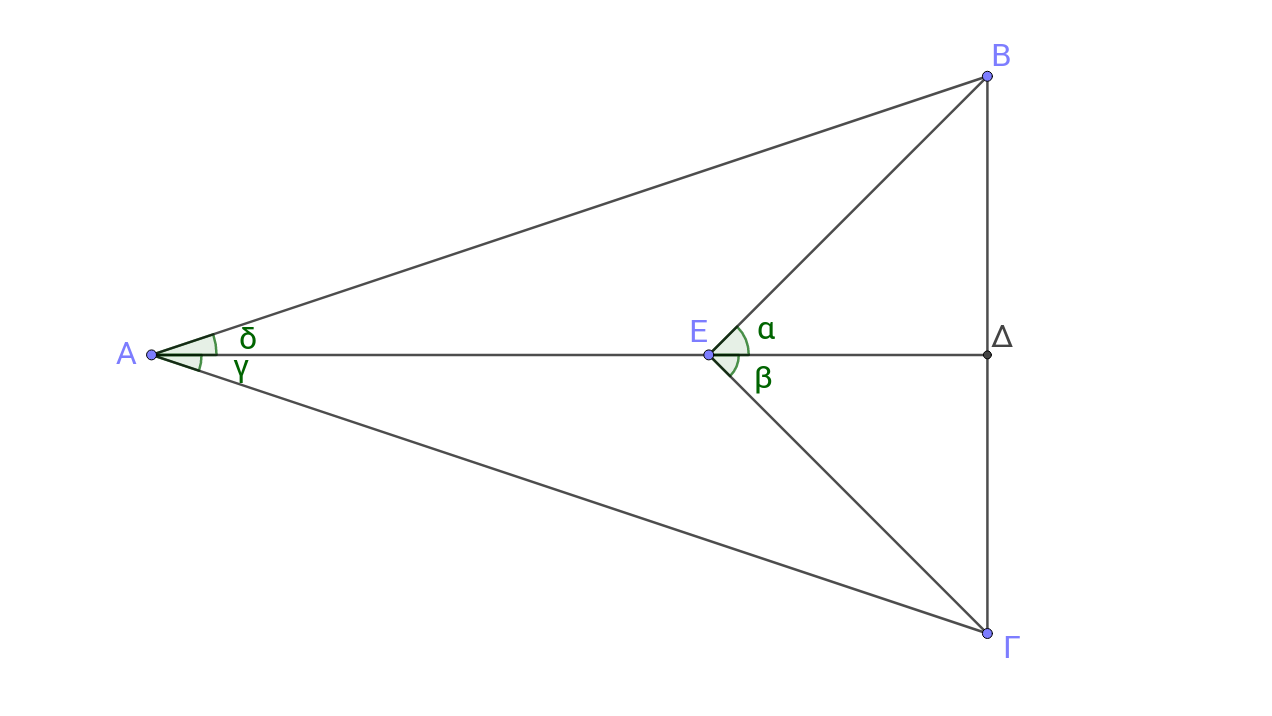
\includegraphics[width=0.5\textwidth]{2017AGeoDiag}
  \end{wrapfigure}
  Αν για το ισοσκελές τρίγωνο $ΑΒΓ$ ($ΑΒ=ΑΓ$) του σχήματος ισχύουν $\hat{α}=\hat{β}$ και $\hat{γ}=\hat{δ}$, να αποδείξετε ότι
  \begin{enumerate}
    \item \textbf{[Μονάδες 11]} Τα τρίγωνα $ΑΕΒ$ και $ΑΕΓ$ είναι ίσα.
    \item \textbf{[Μονάδες 11]} Το τρίγωνο $ΓΕΒ$ είναι ισοσκελές.
    \item \textbf{[Μονάδες 11]} Η ευθεία $ΑΔ$ είναι μεσοκάθετος του τμήματος $ΒΓ$.
  \end{enumerate}
  %\vspace{7\baselineskip}

\section*{Θέμα Γ}
  \noindent
  Δίνεται τρίγωνο $ΑΒΓ$ με $ΑΒ<ΒΓ$. Στην προέκταση της $ΑΒ$ προς το $Β$ παίρνουμε σημείο $Ε$ ώστε $ΑΕ=ΑΓ$. Στην πλευρά $ΑΓ$ θεωρούμε σημείο $Δ$ ώστε $ΑΔ=ΑΒ$. Αν τα τμήματα $ΔΕ$ και $ΒΓ$ τέμνονται στο $Κ$ και η προέκταση της $ΑΚ$ τέμνει το $ΕΓ$ στο $Μ$. Να αποδειχθεί ότι:
  \begin{enumerate}
    \item \textbf{[Μονάδες 8]} $ΒΓ=ΔΕ$
    \item \textbf{[Μονάδες 8]} $ΒΚ=ΔΚ$
    \item \textbf{[Μονάδες 9]} Η $ΑΚ$ είναι η διχοτόμος της $\hat{Α}$.
    \item \textbf{[Μονάδες 9]} Η $ΑΜ$ είναι η μεσοκάθετη του $ΕΓ$.
  \end{enumerate}

\vspace{3\baselineskip}

\part*{\centering{Καλή επιτυχία}}

\end{document}
